\documentclass{beamer}
\usetheme{metropolis}

\usepackage{pgfpages}
\usepackage{xcolor}
\usepackage{pifont}
\usepackage{minted}

%\setbeameroption{hide notes} % Only slides
%\setbeameroption{show only notes} % Only notes
\setbeameroption{show notes on second screen=right}

\title{Keep Your Laziness In Check}
\author{\textbf{Kenny Foner}, \textbf{Hengchu Zhang}, and \textbf{Leo Lampropoulos}}
\institute{University of Pennsylvania}
\date{November 20, 2017}

\definecolor{forestgreen}{rgb}{0.0, 0.75, 0.13}
\newcommand{\greentick}[0]{\color{forestgreen}\ding{51}}
\newcommand{\redcross}[0]{\color{red}\ding{55}}

\begin{document}
\frame{\titlepage}

\begin{frame}
\frametitle{Being lazy is fun and useful, but\dots}
\Large\dots sometimes it leads to unintended consequences.
\end{frame}

\iffalse
\begin{frame}[fragile]
\frametitle{Amortized queues have strange laziness}
\begin{minted}{haskell}
enQ a (front,     back) =
      (front, a : back)

deQ ([],         [])   = Nothing
deQ (a : front', back) = Just (a, (front', back))
deQ ([],         back) = Just (a, (front', []))
  where
    (a : front') = reverse back
\end{minted}
\end{frame}

\note[itemize]{
  \item The usual implementation of functional queues uses two lists: when an
        item is enqueued, it is cons'ed onto the back list, and when we dequeue,
        an item is taken from the head of the front list. When the front list
        becomes empty, the back queue is reversed and takes the role of the new
        front list.
  \item This has amortized O(1) performance cost.
  \item This queue is lazy as long as you don't empty the front, then it is
        fully lazy in the structure of the back list. It only forces the spine
        of the back list when the front list is emptied.
}

\begin{frame}
\frametitle{But it doesn't have to be this way!}
\large
Chris Okasaki:\\
``Simple and Efficient Purely Functional Queues and Deques''
\vspace{.5\baselineskip}\\
(\emph{Journal of Functional Programming}, October 1995)
\end{frame}
\fi

\note[itemize]{
\item Kenny:
\item Enqueue O(1), Dequeue O(1) NOT AMORTIZED because of laziness!
\item Guarantees valid persistently; thunks are only evaluated once
\item How do we know we have implemented the Okasaki Queues correctly?
\item Correctness != functional correctness or micro-benchmark performance:
\item == the right amount of lazy
}

\begin{frame}
\frametitle{Wouldn't it be nice to QuickCheck laziness?}
Traditional property-based testing (such as QuickCheck):
\begin{itemize}
\item[\greentick] Great for testing functional correctness
\item[\greentick] Write a specification, fuzz inputs to functions to automatically test against that specification
\item[\redcross] Can't observe (or even specify) properties beyond functional correctness
\end{itemize}
If we were able to \textbf{specify} and \textbf{observe} laziness, we could
treat it \emph{just like} functional correctness.
\end{frame}

\note[itemize]{
\item QuickCheck gives functional correctness
\item But laziness can't be observed by QuickCheck
\item What if we make it observable? Then it's just part of functional correctness!
}

\begin{frame}
%\frametitle{Introducing: StrickCheck}
\Huge\centering\textbf{StrictCheck}\vspace{.15\baselineskip}\\
\Large\centering``We actually can do that thing.''
\end{frame}

\begin{frame}[fragile]
\frametitle{Observing strictness (part I)}
\begin{minted}{haskell}
instrumentListWithRef :: IORef Int -> [a] -> [a]
instrumentListWithRef _     []       = []
instrumentListWithRef count (a : as) =
  unsafePerformIO $ do
    modifyIORef' count (\x -> x + 1)
    return (a : instrumentListWithRef count as)
\end{minted}
\end{frame}

\note[itemize]{
\item Hengchu:
\item \texttt{instrumentListWithRef} injected a snippet of code at every cons cell
\item and it returns a new ``loaded'' list
\item the injected code is executed as the ``loaded'' list gets pattern-matched on
}

\begin{frame}[fragile]
\frametitle{Strictness doesn't exist in a vacuum}

\begin{itemize}
\setlength\itemsep{-0.5em}
\item<1->[]
\begin{minted}{haskell}
type Context a = a -> ()
\end{minted}
\item<2->[]
\begin{minted}{haskell}
-----------------------------------------------
lazy, whnf, spineStrict :: Context [a]
lazy        = \xs -> const () xs
\end{minted}
\item<3->[]
\begin{minted}{haskell}
whnf        = \xs -> case xs of
                       []    -> ()
                       (_:_) -> ()
\end{minted}
\item<4->[]
\begin{minted}{haskell}
spineStrict =
  \xs -> whnf (foldl' (\ys y -> y : ys)) [] xs)
\end{minted}
\end{itemize}
\end{frame}

\note[itemize]{
  \item The context type gives a function that returns a trivial value of the
        unit type
  \item It might look like there's only one such function \texttt{const ()}
  \item There can actually be all kinds of varying strictness behavior
  \item Forcing the unit value triggers the strictness behavior on the input \texttt{a}
  \item This gives us an easy way to observe the strictness behavior of a context
}

\begin{frame}[fragile]
\frametitle{Demanding an answer, lazily}
\begin{itemize}
\item<1->[]
\begin{minted}{haskell}
evaluate :: () -> IO ()
evaluate () = return ()
\end{minted}
\item<2->[]
\begin{minted}{haskell}
demandCount :: Context b -> ([a] -> b) -> [a] -> Int
demandCount c f as =
  unsafePerformIO $ do
    count <- newIORef 0
    let observableList =
          instrumentListWithRef count as
    evaluate ((c . f) observableList)
    readIORef count
\end{minted}
\end{itemize}
\end{frame}

\note[itemize]{
  \item The seemingly trivial evaluate function forces the unit value returned
        by a context, thus triggering evaluation of the demanded part of
        observableList
  \item \texttt{demandCount} takes a context, and a function that operates over
        lists and the input list
  \item it applies instrumentListWithRef on the input list, producing an
        observableList, and applies the function and context over the
        observableList, triggering the injected instrumentation code
}

\begin{frame}[fragile]
\frametitle{Examples of \texttt{demandCount}}
\begin{itemize}
\item<1->[]
\begin{verbatim}
ghci> let f = take 6
\end{verbatim}
\item<2->[]
\begin{verbatim}
ghci> demandCount lazy f [1..5]
\end{verbatim}
\item<3->[]
\begin{verbatim}
0
\end{verbatim}
\item<4->[]
\begin{verbatim}
ghci> demandCount whnf f [1..5]
\end{verbatim}
\item<5->[]
\begin{verbatim}
1
\end{verbatim}
\item<6->[]
\begin{verbatim}
ghci> demandCount spineStrict f [1..5]
\end{verbatim}
\item<7->[]
\begin{verbatim}
5
\end{verbatim}
\end{itemize}
\end{frame}

\note[itemize]{
\item Just some examples showing demandCount
\item Note that we simply treat \texttt{f} as a black box
\item We don't need to know anything more about \texttt{f} other than the fact
      it typechecks with demandCount!
}

\begin{frame}[fragile]
\begin{columns}
\begin{column}{0.7\textwidth}
\frametitle{Beyond lists and numbers}
\begin{figure}
\centering
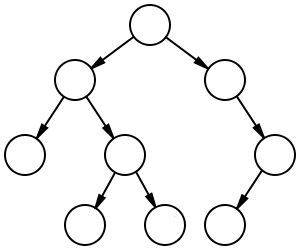
\includegraphics[width=0.7\textwidth]{binary-tree}
\end{figure}
\end{column}
\begin{column}{0.2\textwidth}
{\fontsize{100}{50}\textrm{\textbf{?}}}
\end{column}
\end{columns}
\end{frame}

\note[itemize]{
\item Kenny:
\item This gives us a bare example that counts the number of cons cells forced,
      but what if we want more fine grained information of arbitrary algebraic
      data types?
\item Numbers can't directly capture the structure of a tree, so it can't
      capture the nodes of a tree that get forced in a computation
}

\begin{frame}[fragile]
\frametitle{\texttt{ListDemand}}
\begin{minted}{haskell}
data List a =
    Cons a (List a)
  | Nil

data Thunk a = T | E a

data ListDemand d =
    ConsD (Thunk d)
          (Thunk (ListDemand d))
  | NilD

data IntDemand = IntD
\end{minted}
\end{frame}

\note[itemize]{
  \item Now, we can exactly characterize the demand on a list of Ints by
        composing the type ListDemand and IntDemand
}

\begin{frame}[fragile]
\frametitle{Examples}
\begin{minted}{haskell}
data ListDemand d =
    ConsD (Thunk d)
          (Thunk (ListDemand d))
  | NilD

data IntDemand = IntD
---------------------------------------------------
ConsD T
  (ConsD (E IntD)
     (ConsD T T))

ConsD (E IntD)
  (ConsD T
    (ConsD (E IntD) (E NilD)))
\end{minted}
\end{frame}

\note[itemize]{
  \item The 2nd Int is forced, and we force 3 cons cells, we don't force
        anything in the rest of the list
  \item The 1st and 3rd Int is forced, and the list's spine is forced
  \item Note that these represent concrete observations instrumented on given
        inputs, they do not represent the general behavior of contexts
}

\begin{frame}[fragile]
\frametitle{\texttt{TreeDemand}}
\begin{minted}{haskell}
data Tree a =
    Node (Tree a) a (Tree a)
  | Leaf

data TreeDemand d =
    NodeD (Thunk (TreeDemand d))
          (Thunk d)
          (Thunk (TreeDemand d))
  | LeafD
\end{minted}
\end{frame}

\note[itemize]{
  \item The demand type for a binary Tree
  \item We can either demand the value at an internal node, or one of the
        subtrees
  \item The demand type represents all of the possible prefixes/subshapes of its
        corresponding data type
}

\begin{frame}[fragile]
\frametitle{\texttt{ListDemand} vs \texttt{TreeDemand}}
\begin{minted}{haskell}
data ListDemand d =
    ConsD (Thunk d)
          (Thunk (ListDemand d))
  | NilD

data TreeDemand d =
    NodeD (Thunk (TreeDemand d))
          (Thunk d)
          (Thunk (TreeDemand d))
  | LeafD
\end{minted}
\end{frame}

\note[itemize]{
\item Notice the similarity between ListDemand and TreeDemand with their
      corresponding data types
\item In general, the demand type of a data type simply interleaves a
      \texttt{Thunk} at every constructor field
}

\begin{frame}[fragile]
\frametitle{Computing demand, generically}
\begin{itemize}
\item<1->[]
\begin{minted}{haskell}
demandList :: Context b -> ([Int] -> b)
           -> [Int]
           -> (b, Thunk (ListDemand IntDemand))

demandTree :: Context b -> (Tree Int -> b)
           -> Tree Int
           -> (b, Thunk (TreeDemand IntDemand))
\end{minted}
\item<2->[]
\begin{minted}{haskell}
-----------------------------------------------
demand     :: Context b -> (a -> b) -> a
           -> (b, Thunk (Demand a))
\end{minted}
\end{itemize}
\end{frame}

\note[itemize]{
\item FIX THE MARGIN ISSUES
\item There is a generic transformation between a data type and its
      corresponding data type representing a demand upon it
\item \texttt{Demand} is a type level function that calculates the demand type
\item We return a \texttt{Thunk} of demand because the input might not be
      demanded at all
\item As the input value is traversed by the function, which is driven by the
      context, the evaluation of each thunk builds a pointer based data
      structure which is isomorphic to the demand data type, which is then
      frozen into a demand representation
}

\begin{frame}[fragile]
\frametitle{Generic \texttt{Demand} calculation}
\begin{minted}{haskell}
type family Demand (x :: *) :: * where
 Demand (a -> b)  = FuncDemand
 Demand (a :+: b) = Demand a :+: Demand b
 Demand (a :*: b) = Thunk (Demand a) :*: Thunk (Demand b)
\end{minted}
\end{frame}

\note[itemize]{
\item For simplicity, we speak of types in terms of sums and products
\item \texttt{FuncDemand} is isomorphic to IntDemand in that it only captures
      whether the function was used at all
}

\begin{frame}[fragile]
\frametitle{First-order specifications}
\begin{minted}{haskell}
-- uncurried take
take     :: (Int, [a]) -> [a]

takeSpec :: Int -> [a]
         -> Demand [a]
         -> (Thunk (Demand Int), Thunk (Demand [a]))
\end{minted}
\end{frame}

\note[itemize]{
  \item Having demonstrated how to reify demand behaviors into value, we now
        need to figure out how to write down a specification to check if whether
        a particular run of the program has the specified laziness according to
        the specification
  \item Specifications goings backwards from demands on the output to demands on
        the inputs of the function. This is because how much input is demanded
        depends on how much output is demanded, hence the arrows go the other
        way.
  \item Note that \texttt{takeSpec} takes the same inputs as \texttt{take}
        would. This is necessary in general because the demand behavior of
        programs can depend on their inputs, as it is the case for
        \texttt{take}!
}

\begin{frame}[fragile]
\frametitle{Connecting specification with observation}
\Huge PLACEHOLDER FOR PICTURE
\end{frame}

\note[itemize]{
  \item To QuickCheck \texttt{takeSpec}, we use mechanisms from QuickCheck to
        fuzz an Int and a [a] as inputs for \texttt{take}
  \item We use the \texttt{CoArbitrary} mechanism to generate random contexts
        that exerts non-trivial demand on the output values of \texttt{take}
  \item We use the generic \texttt{demand} function to kick off the entire
        computation
  \item We have now observed the demand on the input and also the demand on the
        output of take, so we can just straightforwardly compare that to what
        the specification expects.
  \item If we find a counterexample, we shrink the inputs first, and then shrink
        the reified demand, and re-exert that new demand on the output.
}

\begin{frame}[fragile]
\frametitle{Higher-order specifications}
\Huge PLACEHOLDER FOR PICTURE
\end{frame}

\note[itemize]{
  \item There is in fact also a mechanical transformation between the type of a
        function to the type of its demand specification
  \item Moreover, this transformation works even with high-order functions
  \item Higher-order specifications will take specification of their input
        functions because their demand behavior is parameterized over the demand
        behavior of their input functions
  \item At testing time, these specifications can be fuzzed through the same
        \texttt{CoArbitrary} mechanism
}

\begin{frame}[fragile]
\frametitle{Contributions}
With \textbf{StrictCheck}, you will be able to:
\begin{itemize}
\item \textbf{Observe} laziness from within Haskell
\item \textbf{Specify} laziness properties as Haskell functions
\item \textbf{Test} implementations against those specifications
\item \textbf{For all types},\footnotemark\, including higher-order functions and
      data types containing functions
\end{itemize}
The implementation is a work in progress.
\footnotetext[1]{Simple (i.e. non-indexed, non-existential) types}
\end{frame}

\note{
StrictCheck is a lightweight tool that adds a very small overhead for
instrumentation and observation of functional programs in Haskell. It also
provides infrastructure for writing specifications and checking
}

\end{document}
